\chapter{Related Work}\label{chap:RelatedWork}

Utilization of zebrafish as a model has received lots of attention in recent year. Advances in imaging technologies and growing number of applications is pressing the need for automated image analysis methods. Table \ref{table:reviewPast} presents the summary of past work for zebrafish analysis. We divided the related work into three sections on the basis of analysis: manual; semi-automated and automated. We further grouped the automated methods based on the type of methods used for analysis.

\section{Manual Analysis}

Arslanova et al. \cite{Arslanova10} developed a method to examine live zebrafish that were each treated with gamma-secretase inhibitors (GSI), DAPT {N-[N-(3,5-difluorophenacetyl-L-alanyl)]-S-phenylglycine t-butyl ester}, Gleevec, or fragments of Gleevec in a zebrafish model of Alzheimer's disease (AD). 


\begin{landscape}
\begin{table}
\caption{Summary Zebrafish Image Analysis} % title name of the table
\centering % centering table
\scalebox{0.85}{
\begin{tabular}{| l | l | l | l | l | l | l |} % creating 10 columns
\hline\hline % inserting double-line
 \textbf{Method} & \textbf{Imaging Modality} & \textbf{Anatomy} & \textbf{Dimension} & \textbf{Application} & \textbf{Analysis Type} & \textbf{Year}
\\ [0.5ex]
\hline % inserts single-line
% Entering 1st row
    Liu et al. & Digital Microscopy & Whole Organism & Gene Expression & 2D & Automated & 2006 \\ \hline
		
    Shirinifard et al. & Confocal & Vasculature & 3D + t & Toxicology & Manual & 2013 \\ \hline
		
		Chen et al. & n.s. & Vasculature & 2D & Gene Expression & Manual & 2005 \\ \hline
		
		Liu et al. & Bright Field & Whole Organism & 2D  & Toxicology & Automated & 2012 \\ \hline
		
		Xu et al. & Bright Field & Torso & 2D & Toxicology & Automated & 2010 \\ \hline
		 
		Arslanova et al. & Microscope & Whole Organism & 2D & Gene Expression & Manual & 2010 \\ \hline
		
		Tran et al. & Fluorescent & Vasculature & 2D & Drug Discovery & Semi Automated & 2007 \\ \hline
		
		Yozzo et al. & Fluorescent & Whole Organism & 2D & Toxicology & Semi Automated & 2013 \\ \hline
		
		Stern et al. & Microscope & Whole Organism & 2D & Toxicology & Automated & 2011 \\ \hline
		
		Kato et al. & CCD Camera & Whole Organism & 2D + t & Behavior pattern & Automated & 2004 \\ \hline
		
		Vogt et al. & Fluorescent & Vasculature & 2D & Toxicology & Automated & 2009 \\ \hline
		
		Feng et al. & Fluorescent & Vasculature & 3D & Toxicology & Automated & 2005 \\ \hline
		
		Chen et al. & Microscope & Whole Organism & 2D & Drug Discovery & Automated & 2011 \\ \hline
		
		Tal et al. & Confocal & Whole Organism & 3D + t & Toxicology & Semi-Automated & 2014 \\ \hline
		
		Kamali et al. & Confocal & Brainstem & 3D & Disease Modeling & Automated & 2009 \\ \hline
		
		Anilla et al. & Fluorescent & Whole Organism & 2D & Disease Modeling & Semi - Automated & 2013 \\ \hline
		
		Mccollum et al. & n.s & Whole Organism & 2D & Toxicology & n.s. & 2011 \\ \hline
		
		Alshut et al. & Microscope & Whole Organism & 2D & Toxicology & Automated & 2010 \\ \hline
		
		Peravali et al. & Microscope & Brain & 2D & n.s. & Manual & 2011 \\ \hline
		
		Bang et al. & CCD Camera & Whole Organism & 2D + t & Behavior pattern & Automated & 2002 \\
		
\hline % inserts single-line
\end{tabular}
\label{table:reviewPast}
}
\end{table}
\end{landscape}

Several GSI are in clinical trials for the treatment of AD. Brain regions (ROI) from the dorsal view images are manually segmented. The intensity of each ROI is quantified. To measure the gene expression, a manual approach is not only time-consuming but also lack objectivity due to inter-observer variations.

Shirinifard et al. \cite{Shirinifard13} discussed quantitative analysis of growth dynamics for characterization of both normal and perturbed growth for ISV. Their method is based on analyzing ISV trajectories (sequences of successive 3D locations over time). Manual Tracking plugin in FIJI ImageJ is used to track 3D position of ISV sprout bases and tips over time (x, y, z coordinates over time). ISV sprout base position is the midpoint of the sprout where it intersects with the DA. ISV tip position is the farthest point on the ISV from the point of attachment on DA. Displacement and angle between the ISV and the DA is used to correct for zebrafish embryos twitching. Average trajectories are calculated for control and for arsenic treated embryo. Average trajectories are fitted with quadratic curve to produce a canonical ISV trajectory.  Curvature, average directed migration speed and directionality were computed from canonical trajectories. Curvature, average directed migration speed and angle between the ISV and DA were different for arsenic treated vs untreated.

Chen at al. \cite{Chen05} proposed to use caudal vein to study the affects of modifications of sulfate 6-O sulfotransferase (HS6ST) genes on zebrafish development. Authors observed formation of large loops with high penetrance for the caudal vein. Quantification is done on the basis of number of embryos showing abnormal caudal vein development. 

In the review done by Mccollum et al. \cite{mccollum2011} explores the questions of using zebrafish as a screening tool for human risk assessment. Toxicity effects on the zebrafish development are reviewed from existing literature. Toxic effects are reported on cardiovascular, somite, muscular, skeletal, and neuronal systems. They also report abnormal behavior, changes in gut, pancreas, liver, and kidney development, as well as toxic effects on the immune system and lipid metabolism. 

Cheng et al. \cite{cheng2001} studied the effects of cadmium on cardiovascular development in zebrafish embryos. They concluded that exposure to cadmium could affect the morphogenesis of the vasculature. In embryos with visible abnormalities, the vasculature in the malformed region correlated well with defective vascular patterning. There is a significant reduction in number of branches for cadmium exposed embryos as compared to health embryos.  


\section{Semi-Automated Analysis} \label{sec:RelatedWorkSemi}

Tran et al. \cite{Tran07} proposed an interactive algorithm using the Discovery-1/MetaMorph software to rapidly analyze each image. ISV is isolated from rest of images, by manually removing trunk from the fluorescent image. ISV is separated from rest of image using mask. The software counts the number of intersegmental vessels and branching arteries in the isolated trunk of the embryo. Manual segmentation of trunk restricts its usage for HTS. As shown in our work certain compounds do not alter ISV count but, end up changing other dynamics of ISV.

Yozzo et al. \cite{Yozzo13} screened 10 known cardiovascular toxicants through an image analysis pipeline that included ISV sprout length quantification. Semi-automated methods are used to isolate regions of interest and quantify heart rate, circulation, pericardial area, and intersegmental vessel area, whereas a fully automated method is used to quantify body length.

Tal et al. \cite{Tal14} tested the effect of environmental chemicals on formation of the vascular system. They developed a quantitative assay in transgenic zebrafish and evaluated the assay using angiogenesis inhibitors that target VEGFR2 (PTK787) or EGFR (AG1478). Both PTK787 and AG1478 exposure impaired ISV sprouting, while AG1478 also produced caudal and pectoral fin defects at concentrations below those necessary to blunt ISV morphogenesis. The functional consequences of vessel toxicity during early development included decreased body length and survival in juvenile cohorts developmentally exposed to inhibitor concentrations sufficient to completely block ISV sprouting angiogenesis. Vascular growth depicted in time-lapse image stacks is quantified in automated manner where as ISV length is manually observed. 

ZebIAT is image analysis tool developed by Anilla et al. \cite{annila2013} that allows both automatic or semi-automatic registration of the outer contour and inner organs of zebrafish embryos. ZebIAT provides a registration at different stages of development and an automatic analysis to study cancer progression. The user manually marks the organs or other areas of interest in the reference zebrafish embryo image. Outline of the zebrafish is obtained by segmentation and edge detection. Landmark based registration is applied to register images to reference image. Labeled cancer cells are detected using a method of multiscale product of wavelet and the mean fraction of the area of each organ that exhibited cancer spots in the embryos is examined.

To enable large scale observations Peravali et al. \cite{peravali2011} developed an algorithm to identify head region from low resolution image based on template matching. The regions of interest are subsequently imaged automatically at high magnification, enabling rapid capture of cellular resolution data. The pixel location in the source image yielding the largest normalized cross-correlation measure was considered the best match between the template and the source image, and is chosen as the center of the field of view for subsequent high-resolution imaging.

\section{Automated Analysis}
This section discuses automated techniques for zebrafish image analysis. Review is grouped into various subsection, based on type of method used for image analysis. Figure \ref{overviewRelatedWrok} gives an overview of algorithm utilized for analysis. It also includes, few of the methods described in section \ref{sec:RelatedWorkSemi}.

\begin{landscape}
\begin{figure}[htb] 
 \begin{center}
    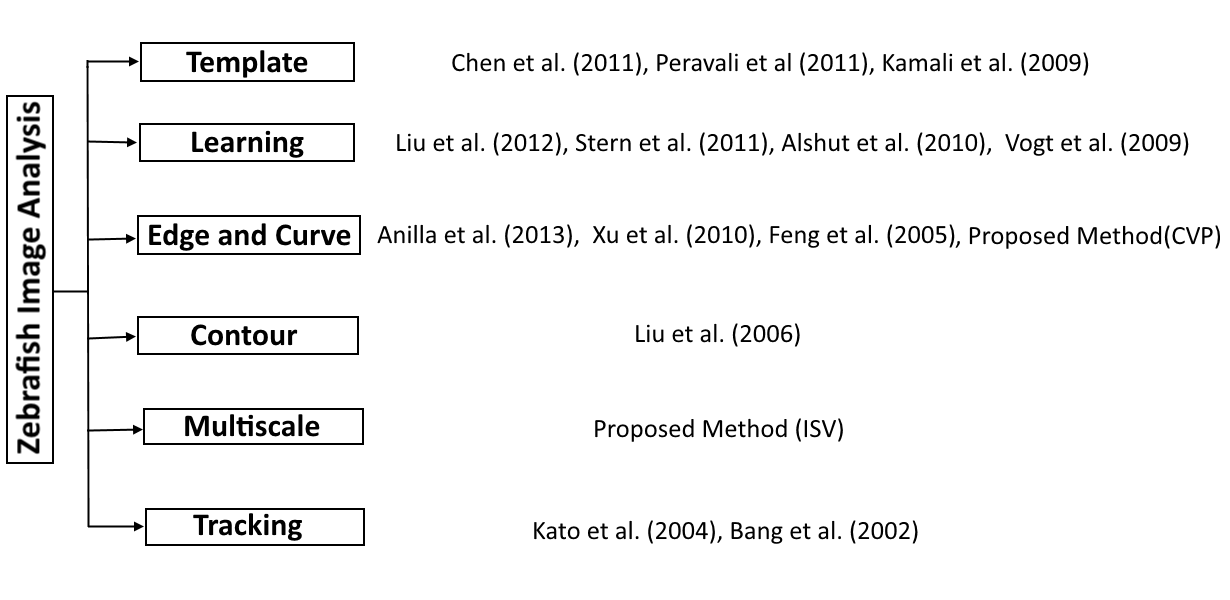
\includegraphics[scale=0.6]{figure/review.png}
  \end{center}
  \caption[Overview of an automated/semi-automated image analysis methods.]{Overview of an automated/semi-automated image analysis methods.}
 \label{overviewRelatedWrok}
\end{figure}
\end{landscape}
\par

\subsection{Template Based}

Chen et al. \cite{Chen11} proposed a robust automatic segmentation to identify ROIs for gene expression quantification. Their pipeline consisted of image alignment, segmentation, extraction and quantification of 15 ROIs. The telencephalon, left and right (L\&R) dorsal diencephalon, L\&R olfactory vesicles, ventral midbrain, L\&R retina, L\&R branchial arches, ventral hindbrain, L\&R dorsal hindbrain, and L\&R pectoral fin is quantified to evaluate gene expression. Size of each of the ROI is calculated for quantification. 

Kamali et al. \cite{kamali2009} developed a 3D template-based tracing algorithm to localize and differentiate the fluorescent neurons. A control template consisting of 28 zones with 14 zones on each side of the brainstem is created as a representation of 300 neurons that descend from the larval zebrafish brain into the spinal cord. The template is initialized by registering neurons manually identified in the different zones. After the creation of the template, image processing steps are applied to detect neurons and assign them to the template. First process is image registration of confocal z-stacks into a normalized space. User select three points on a MIP projection of confocal z-stack and corresponding points on template. Affine transform is applied to the 3D image stack to register it to the template. Second process of segmentation involves two steps: (1) neurons are segmented on each xy - plane to find a set of intensity contours with appropriate size and shape so as to reveal each neuronal cell body present in the plane (2) segmented results over consecutive xy-plane images are associated with the same neurons based on the assumption that each neuron spans several images along the z-direction. Lastly, for cell identification template is used in conjunction with the segmented boundary contours to assign detected neurons to specific zones and sub-zones of the brainstem.

\subsection{Learning Based}

Liu et al. \cite{Liu12} proposed a recognition model for high throughput screening of toxicity based on image descriptors based on color and texture combined with a support vector machine to recognize three basic phenotypes (hatched, unhatched, and dead). The best performing model is attained with three image descriptors (color histogram, representative color, and color layout) identified as most suitable from an initial pool of six descriptors. The SVM classification model is developed using the three descriptors: (a) Global and Semi-global Edge Histogram Descriptor (GSEHD), (b) Representative Color Descriptor (RCD), and (c) Color Histogram Descriptor (CHD). They reported an average classification accuracy of 97.40±0.95\% in a 10-fold cross-validation and 93.75\% classification accuracy for a stress test with zebrafish images of low quality. This system can be used to identify extreme cases of toxicity, but further analysis is needed to identify less extreme cases.

Alshut et al. \cite{alshut2010} proposed learning based classification approach, which detects the embryo in the well, classifies its status and derives characteristic parameters for the regions. Expert labeled the data to the classes dead, alive or unknown. Chorion is segmented from background using adaptive threshold and features are derived based on intensity edge filter, and chorion size. Two most discriminative features are selected by MANOVA (multivariate analysis of variances). Using these two features, the classification is performed utilizing a Bayesian classifier.

Stern et al. \cite{Stern11} focused on automatically detecting specific interest points in microscopy images. Images are manually annotated by expert to identify interest points coordinates and to train models able to predict those interest points in new, unseen images. The approach first extracts sub-windows (or patches) around points of interest and at other randomly chosen positions within images. The patches are described by various visual features, RGB, HSV, Grayscale, Edge strength, Local Binary Pattern. A classification or a regression model is built using these features. In the classification scheme, the model is trained to predict whether the central pixel of a sub-window is an interest point or not (a binary classification problem). In the regression scheme, the model predicts the distance between the central pixel of a sub-window and the interest point.

Vogt et al. \cite{Vogt09} implemented a user guided image interpretation tool to generate rule-based hierarchical image segmentation. The zebrafish embryos are first segmented, and the large vessels and head structures are identified based on pixel values. The algorithm then removes small and isolated objects. Next, the remaining regions are re-processed to identify the head, dorsal aorta, and posterior cardinal vein. These pre-processed images were then used for blood vessel quantification. Numerical measurements of blood vessels development such as area, length, and shape are captured. 

\subsection{Contour Based}

Liu et al. \cite{Liu06} have proposed to automatically quantify the neurons and somites in a large number of zebrafish images, as well as quantitative measurement of gene expression levels in zebrafish embryos. Neurons are segmented from edge image using circular Hough transform. Rohon–Beard (RB) sensory neurons are segmented using method based on intensity projection. Somites are recognized using gray level co-occurrence matrix, and edge direction histogram. ROI for genes quantification is established with region growing segmentation. Neurons quantification is based on its count. There is neuron loss in zebrafish embryos due to knockdown of AD-linked genes. Somites are quantified using features extracted from gray level co-occurrence matrix for detection of defective somites.

\subsection{Curvature and Edge Based}

Xu at al. \cite{Xu10} proposed an algorithm focused on detecting and quantifying pigments in zebrafish embryos. They automatically identify torso area through series of image processing steps. Steps include, finding single zebrafish in an image and then rotating the images so the embryo is positioned with its head region to the upper right corner and with its back pointing upward and abdomen downward to allow the algorithm to search the abdominal region based on the zebrafish anatomy. A watershed method is used to remove the head region from the torso that contains the pigmentation. Otsu’s method is applied on the torso for segmentation, which is quantified and used for toxicology. 

Feng et al. \cite{Feng05} developed a 3D attributed vessel represent graph (AVRG) approach to reconstruct caudal vasculature of zebrafish embryo. The major steps of the framework include pre-processing, vasculature reconstruction, vascular structure quantification, and presentation. Pre-processing steps for vessel segmentation include: (1) Image enhancement; (2) Adaptive thresholding; (3) Vessels registration; (4) Edge tracking and curve fitting. The cross-sections of a segmented vessel are represented by ellipses. The surface of a blood vessel is represented by triangle meshes. Vasculature structure is reconstructed by locating junction points at the intersections of two or more vessels. Reconstructed vasculature structure is then utilized for quantification of the number and connectivity of the vessels, their size, length, and volume, as well as the distance between any two vessels.


\subsection{Tracking Based}

Bang et al. \cite{bang2002} developed an automated screening assay to detect hearing defects in zebrafish by monitoring their behavior after receiving a loud sound burst. The image was acquired immediately before the tone burst was subtracted from the image acquired immediately after the tone burst. If the zebrafish did not respond to the tone burst, due to hearing defects, the subtraction of its images produced an image approximating zero. If the zebrafish responds to the tone burst by moving to a different position, the subtraction result contains both positive and negative pixel values that can be detected by taking the absolute value of the resulting image and segmenting it by an appropriate threshold.

Kato et al. \cite{Kato04} developed computer image processing system for quantifying zebrafish behavior. Zebrafish images were extracted in real time from the original image as a binary image by removing a background of the aquarium before the fish are introduced. To maintain an effective frame rate that is high enough to capture the movement of the zebrafish, skipping search method is applied on data. In each frame, only one fourth of the pixels are \textquotedblleft skippingly\textquotedblright examined, and then only the areas of interest that are recognized as zebrafish are analyzed in more detail in the two diagonal directions and in two crosswise directions with a continuous search. Chasing behavior of pairs of fish are quantitatively analyzed based on the positional coordinates of their center of gravity.

\begin{figure}[htb] 
 \begin{center}
    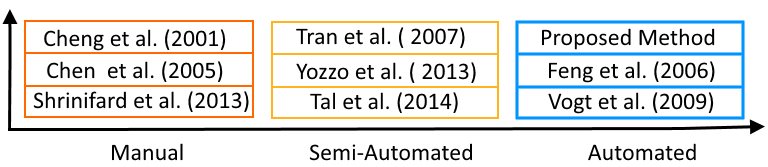
\includegraphics[scale=0.65]{figure/analysisReview.png}
  \end{center}
  \caption[Overview of vasculature image analysis methods]{Overview of vasculature image analysis methods.}
 \label{analysis}
\end{figure}

\begin{figure}[htb] 
 \begin{center}
    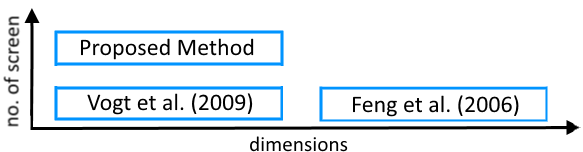
\includegraphics[scale=0.85]{figure/automatedReview.png}
  \end{center}
  \caption[Overview of an automated vasculature image analysis methods]{Overview of an automated vasculature image analysis methods.}
 \label{automated}
\end{figure}



\par
Automated analysis of vasculature is still a budding field. Feng \cite{Feng05}, and Vogt \cite{Vogt09}, and proposed method are the only studies dedicated to automated analysis of vasculature blood vessel (fig. \ref{analysis}).  The work presented in their papers has been performed on limited number of compounds (fig. \ref{automated}); there is still a question about its scalability. Feng \cite{Feng05} performed 3d reconstruction of few vessels, where in our work we capture the dynamics of all ISVs. In this work, we have proposed a segmentation and quantification algorithm for ISV and CVP. Segmentation is a very crucial and important step for any kind of analysis. Interestingly, an automatic segmentation of ISV and CVP is still an untouched problem. Segmentation based either on thresholding or on edge detection of images are not sufficient to analyze ISV. ISV are highly diverse; they differ in size, shape, intensity, and occluded with noise. The orientation and amount of details of each embryo are different. One image has multiple embryos placed in various orientations. %(Show image for data issue0) 
To quantify different regions, manual analysis requires one to draw ROIs for every image and then measure the features in each ROI. Often a human observer needs to rotate the images to the same orientation before drawing ROIs and quantifying pixel intensity, making their laborious work more tedious. In addition, manual analysis is subject to inter-observer variation and lacks repeatability.
\par
In summary, although methods have been developed to process zebrafish images, as the applications of the zebrafish model expands, there is a demand for a variety of automated image processing algorithm. In this work we have presented a techniques and a framework for segmentation, representation, quantification and classification of the zebrafish ISV and CVP from  images. The methodology presented is quantitative, can be utilized with wide varieties of toxin treated zebrafish, and capable of quantifying changes in fine structure not quantifiable by the human eye. Relevance of our work is further amplified, by having a model to be able to determine safe dosages for assays of compounds. In next few chapters we will present detailed description of our approach.

